%++++++++++++++++++++++++++++++++++++++++
\documentclass[a4paper,11pt]{article}
\usepackage{url}
\usepackage{hyperref}
\usepackage{amsmath,amssymb}
\usepackage{fullpage}
\usepackage{booktabs}
\usepackage{graphicx}
\usepackage{wrapfig}
\usepackage{caption}
\usepackage{float}
\usepackage{subcaption}
\usepackage{enumerate}
\usepackage{color}
\usepackage{capt-of}
\usepackage{todonotes}
\usepackage{geometry}
 \geometry{
   a4paper,
   total={170mm,257mm},
   left=15mm,
   right=15mm,
   top=15mm,
 }
\usepackage{indentfirst}
  \setlength{\parindent}{0.5em}
  \setlength{\parskip}{0.1em} 
\usepackage{tabularx} % extra features for tabular environment
\usepackage{amsmath}  % improve math presentation
\newcommand{\Test}[1]{\expandafter\hat#1}
\usepackage{graphicx} % takes care of graphic including machinery
\hypersetup{
    colorlinks=true,       % false: boxed links; true: colored links
    linkcolor=blue,        % color of internal links
    citecolor=blue,        % color of links to bibliography
    filecolor=magenta,     % color of file links
    urlcolor=blue
}

% other packages
\usepackage{listings} % code listings
\lstset{framextopmargin=0pt,frame=lines}
\lstset{
	language=Matlab,
    basicstyle=\footnotesize\ttfamily,
    breaklines=true,
    tabsize=4,
    keepspaces=true,
    columns=flexible,
    % backgroundcolor=\color[gray]{0.9},
    frame=single,
    breaklines=true,%
    morekeywords={matlab2tikz},
    keywordstyle=\color{blue},%
    morekeywords=[2]{1}, keywordstyle=[2]{\color{black}},
    identifierstyle=\color{black},%
    stringstyle=\color{mylilas},
    commentstyle=\color{mygreen},%
    showstringspaces=false,%without this there will be a symbol in the places where there is a space
    numbers=left,
    numberstyle={\tiny \color{black}},% size of the numbers
    numbersep=9pt, % this defines how far the numbers are from the text
    emph=[1]{for,end,break},emphstyle=[1]\color{red}, %some words to emphasise
    %emph=[2]{word1,word2}, emphstyle=[2]{style},    
}
\usepackage{color} %red, green, blue, yellow, cyan, magenta, black, white
\definecolor{mygreen}{RGB}{28,172,0} % color values Red, Green, Blue
\definecolor{mylilas}{RGB}{170,55,241}

\usepackage{todonotes}
\usepackage[toc,page]{appendix}
\usepackage{csquotes}


%++++++++++++++++++++++++++++++++++++++++

\begin{document}
\title{
    System Identification \\
    Final Project: Identification of a Torsional System
}
\author{Camilla Carta \\ Michael Spieler}
\date{\today}
\maketitle


\section{Introduction}
For this project, the goal was to identify a linear parametric model for the system showed in Figure \ref{fig:system}. This system consists in a torsional device, that was described in the project assignment as follows:
\begin{displayquote}
\textit{The plant consists of three disks supported by a torsionally flexible shaft which is suspended vertically on anti-friction ball bearings. The shaft is driven by a brushless servo motor connected via a rigid belt (negligible tensile flexibility) and pulley system with a 3 : 1 speed reduction ration. An encoder located on the base of the shaft measures the angular displacement of the first disk. The second disk is connected to its encoder by a rigid belt/pulley with a 1 : 1 speed ratio. The input of the system is the voltage of the servo motor and the output is the position of the third disk.}

\textit{An unknown digital controller is used to control the position of the third disk. A closed-loop experiment has been carried out in which a PRBS signal, r(k), is applied as the reference position and the input to the plant, u(k), as well as the output of the plant, y(k), are measured and saved in FPdata.mat, which is available in Moodle.
The sampling period is $T_s = 0.04s$. The objective is to identify a parametric model for the torsional plant (between u and y) and validate it using different methods.} 
\end{displayquote}

The plant input signal u(k) consisted in a PRBS of size 6138, with 6 periods and a n-bit shift register of 10 bits. With a sampling period of $T_s = 0.04s$, the system was excited for a period of over 4 minutes.

\begin{figure}[H]
\centering
\includegraphics[height = 8cm]{images/torsionalsystem}
\caption{The torsional device to be identified}
\label{fig:system}
\end{figure}

\section{Frequency domain model identification}
%\todo[inline]{Identify a nonparametric frequency-domain model for the system using two different methods : Fourier analysis and spectral analysis using a window.}

\subsection{Fourier analysis}
In order to identify the frequency-domain model of the system, the Fourier analysis was first applied. An averaging was applied to the Fourier Transforms of input and output, as it improves the results' accuracy. The corresponding bode diagram is shown in Figure \ref{fig:bode_model}. Figure \ref{fig:bode_io} shows the bode diagram of the Fourier Transforms for the input and the output respectively. It can be seen that the two resonance frequencies in the model correspond to the resonance frequencies of the input u, while the lowpass effect can be found in the Fourier Transform of the output.


\begin{figure}[H]
\centering
\begin{subfigure}[t]{0.45\textwidth}
  \centering
  \includegraphics[height = 7cm]{images/2_Fourier_analysis}
  \caption{Bode diagram for input and output signals}
  \label{fig:bode_io}
\end{subfigure}
~\qquad \qquad
\begin{subfigure}[t]{0.45\textwidth}
  \centering
  \includegraphics[height = 7cm]{images/1_Fourier_analysis}
  \caption{Bode diagram for the identified model using Fourier analysis and averaging}
  \label{fig:bode_model}
\end{subfigure}

\caption{Fourier Analysis}
\label{fig:FA}
\end{figure}


\subsection{Spectral analysis}

Next, the spectral analysis was performed. In order to improve the accuracy of the results, averaging was applied as in the course notes at page 56. The estimation for a closed-loop system with excitation at the reference signal $r$ needs to be applied, as shown on page 60 in the coruse notes.

\begin{equation}
G(e^{j\omega_n}) = \frac{\bar{\Phi}_{yr}(\omega_n)}{\bar{\Phi}_{ur}(\omega_n))} 
\end{equation}
where
\begin{align}
\bar{\Phi}_{ur}(\omega_n) =\frac{1}{m} \sum_{i=1}^{m} \phi_{ur,i}(\omega_n)
&\qquad\qquad
\bar{\Phi}_{yr}(\omega_n) =\frac{1}{m} \sum_{i=1}^{m} \phi_{yr,i}(\omega_n)
\end{align}
for m equal to the number of periods in the signal. 

Moreover, a windowing was applied on every period of the Fourier Transform in order to remove disturbances. Both Hann and Hamming windows were tested, but the results given were very similar. As such, it was chosen to show only the results for Hann windowing. 

The window size M must be chosen carefully as it is important to keep all the significant part of the signal: in Figure \ref{fig:SA} the effects for different window sizes can be observed. For a window too small (as in Figure \ref{fig:bode_sa_m200}) the curve is smooth but the peaks at the resonance frequencies are lost. On the other hand, for a window too big (as in Figures \ref{fig:bode_sa_m650} and \ref{fig:bode_sa_m2046}) the peaks are maintained but the noise is not attenuated sufficiently. In particular, Figure \ref{fig:bode_sa_m2046} shows that a window with the same size as the period of the Fourier Transform to which it is applied gives results that are very similar to the ones obtained with the fourier analysis (see Figure \ref{fig:FA}).

\begin{figure}[H]
\centering
\begin{subfigure}[t]{0.45\textwidth}
  \centering
  \includegraphics[height = 7cm]{images/1_Spectral_analysis_m200}
  \caption{M = 200}
  \label{fig:bode_sa_m200}
\end{subfigure}
~\qquad \qquad
\begin{subfigure}[t]{0.45\textwidth}
  \centering
  \includegraphics[height = 7cm]{images/1_Spectral_analysis_m550}
  \caption{Bode diagram for the identified model using Fourier analysis and averaging}
  \label{fig:bode_sa_m550}
\end{subfigure}
~
\begin{subfigure}[t]{0.45\textwidth}
  \centering
  \includegraphics[height = 7cm]{images/1_Spectral_analysis_m650}
  \caption{Bode diagram for input and output signals}
  \label{fig:bode_sa_m650}
\end{subfigure}
~\qquad \qquad
\begin{subfigure}[t]{0.45\textwidth}
  \centering
  \includegraphics[height = 7cm]{images/1_Spectral_analysis_m2046}
  \caption{Bode diagram for the identified model using Fourier analysis and averaging}
  \label{fig:bode_sa_m2046}
\end{subfigure}

\caption{Spectral Analysis results with averaging and different values of windowing. We observe two resonance frequencies $\omega_1 \approx 14.1 s^{-1} $ and $\omega_2 \approx 26.6 s^{-1}$}
\label{fig:SA}
\end{figure}

Observing the results, a window of size $M = 550$ can be chosen. The choice was validated using the correlation and the deconvolution approaches to reconstruct the impulse response, which can be seen in Figure \ref{fig:impulse_resp}.


\begin{figure}[H]
\centering
\includegraphics[width = 10cm]{images/1_impulse_response}
\caption{Reconstructed impulse response using correlation and deconvolution approach. The length of the settling time should correspond to the half size of the window $M/2$ which is about 250. This verifies window size chosen above.}
\label{fig:impulse_resp}
\end{figure}

\section{System structure}
%\todo[inline]{Estimate the structure of the system. Give several reasons for your choices (Physical model, frequency response, loss function evolution, zero-pole cancellation, first coefficients of the numerator polynomial).}

In this section, different methods to select the order of the system were tested, as the First Principle modeling, the loss function method, the zero-pole cancellation method and the study of the first coefficients of the numerator polynomial.

\subsection{Physical model}
The physical model consists of 3 disks with different inertias connected in series by two torsionally flexible shafts acting as springs ($k_1$ and $k_2$). The first disk is driven by a electric motor with a torque $T = k_m u$ with $u$ as input voltage. The output of the plant is the angle of the last disk $\theta_3$. This model is illustrated in \ref{fig:plantmodel}.

\begin{figure}[H]
\centering
\includegraphics[width = 8cm]{images/plantmodel}
\caption{Physical plant model}
\label{fig:plantmodel}
\end{figure}

\paragraph{Transfer function}
We can describe the dynamics of the above system as follows
\begin{align}
T = k_m u \\
J_1\ddot{\theta_1} + k_1(\theta_1 - \theta_2) &= T \\
J_2\ddot{\theta_2} + k_1(\theta_2 - \theta_1) + k_2(\theta_2 - \theta_3) &= 0 \\
J_3\ddot{\theta_3} + k_2(\theta_3 - \theta_1) &= 0
\end{align}
We solve for $G = \frac{\theta_3}{u}$
\begin{equation}
G =
k_1 k_2 k_m  \frac{1}{s^2}\frac{1}{J_1 J_2 J_3 s^4 + (J_1 J_2 k_2  + J_1 J_3 k_1  + J_1 J_3 k_2) s^2 + J_2 J_3 k_1  s^2 + J_1 k_1 k_2  + J_2 k_1 k_2  + J_3 k_1 k_2 }
\end{equation}

which we can reformulate as a system with double integrator. We can manually fit the values for $k \approx 10$ and the two resonance frequencies $\omega_1 \approx 14.1 s^{-1} $ and $\omega_2 \approx 26.6 s^{-1}$

\begin{equation}
G = \frac{k}{s^2 (\frac{s^2}{\omega_1^2} + 1)(\frac{s^2}{\omega_2^2} + 1)}
\end{equation}

\begin{figure}[H]
\centering
\includegraphics[width=\textwidth]{images/2_physical_model_fit}
\caption{The bode plot to the left shows the above model manually fit to the spectral-analysis result. The one to the right is the same model but with a double high-pass filter with cutoff $\omega_c = 1.71s^{-1}$ and $k = 3.16$. The right model has a better fit in lower frequencies and also correct phase.}
\label{fig:physical_model_fit}
\end{figure}

Both models shown in Figure \ref{fig:physical_model_fit} are of degree 6, which serves as an indication of the degree of the real model.

Remark: We would expect a double integrator, which comes from the fact that the control input is a torque resulting in an acceleration while the output is a position. The two resonance frequencies come from the two spring-mass systems in series. One frequency is the two inertias in phase and the other in anti-phase.

\paragraph{State-space model} We can also write the dynamical system above as a state-space model:

% \begin{align}
% \dot{x} = Ax+Bu \\
% y = Cx + Du
% \end{align}

\begin{equation}
x =
%\left(\begin{array}{c} \theta_1\\ \theta_2\\ \theta_3\\ \dot{\theta_1}\\ \dot{\theta_2}\\ \dot{\theta_3} \end{array}\right)
\left(\begin{array}{cccccc}\theta_1 &\theta_2 &\theta_3 &\dot{\theta_1} &\dot{\theta_2} &\dot{\theta_3}\end{array}\right)^\intercal
\end{equation}

% use matlab command latex(A)...
\begin{equation}
\dot{x} = 
\left(\begin{array}{cccccc} 0 & 0 & 0 & 1 & 0 & 0\\ 0 & 0 & 0 & 0 & 1 & 0\\ 0 & 0 & 0 & 0 & 0 & 1\\ -\frac{k_1}{J_1} & \frac{k_1}{J_1} & 0 & 0 & 0 & 0\\ \frac{k_1}{J_2} & -\frac{k_1 + k_2}{J_2} & \frac{k_2}{J_2} & 0 & 0 & 0\\ 0 & \frac{k_2}{J_3} & -\frac{k_2}{J_3} & 0 & 0 & 0 \end{array}\right)
x
+
\left(\begin{array}{c} 0\\ 0\\ 0\\ \frac{k_m}{J_1}\\ 0\\ 0 \end{array}\right)
u
\end{equation}

\begin{equation}
y =
\left(\begin{array}{cccccc}0&0&1&0&0&0\end{array}\right)
x = \theta_3
\end{equation}

This means that we can expect to identify a state-space model for the plant with an order of about 6.

Note: We assume that friction is negligible. In the real system there is viscous friction, which would result in non zero values in the diagonal of the lower right part of the matrix A. Though the hypothesis of zero viscous friction is plausible, since we are operating in air at small amplitudes around $\dot{\theta_3} = 0$. We also neglect dry friction, which would add some non-linearities. This is reasonable, since the axis are fixed with low friction ball bearings.


\subsection{Parametric identification methods}
\paragraph{Estimation of $n$ by the loss function}  First, the loss function method for an ARX was applied as explained in the course book at page 109-110. The order of delay $n_k$ was fixed to 1 and $n_a = n, n_b = n$ were increased in a range $1 : 25$. A global criterion was established with a penalty term of type BIC which is given by
\begin{equation}
BIC = L_f(n,N) + \frac{n\log{N}}{N}
\label{eq:bic}
\end{equation}
The results can be seen in Figure \ref{fig:loss_funct_1}. The minimum of the global function gives an order of $n = 5$.

\begin{figure}[H]
\centering
\includegraphics[width = 10cm]{images/1_loss_funct_order}
\caption{Loss function for the ARX model. Estimated order is $n = 5$}
\label{fig:loss_funct_1}
\end{figure}

\paragraph{Zero-Pole cancellation method}
The estimation made above had to be validated. To do this, the zero-pole cancellation method was applied for $n_k = 1$ and $n_a = n_b = n_c = n$ for $n = 1:n_{max}$, where $n_{max}$ was chosen equal to 9 and then the orders were applied to an ARMAX structure. The results can be seen in Figure \ref{fig:zpc}.
As the system is subjected to noise, an exact zero-pole cancellation is impossible; as such, the 95\% confidence intervals corresponding to $\pm2\sigma$ was plotted as well. It was noticed that a zero-pole cancellation occurs for $n = 7$, so the order of the model can be estimated to be 6. The underestimation of the loss function method could be due to a too strong penalty term, as such the zero-pole cancellation estimation is preferred.

\paragraph{Delay estimation}
Once the order of the system was fixed, the delay $n_k$ was estimated. To do this, the first coefficients of $B(q^{-1})$ for a FIR structure have to be evaluated. Then, the \texttt{arx} command was applied for $n_a = 0$, $n_b = n$, in order to create a FIR structure. As explained in the course notes at page 111-112, one has to enumerate the first coefficients equal to 0 or that can be considered 0, as to say if 
\begin{equation}
0 \in [b_k - 2\sigma_k, b_k + 2\sigma_k]
\end{equation}
As it can be seen in Figure \ref{fig:est_delay}, it can be stated that the delay $n_k$ can be estimated equal to 0.

\begin{figure}[H]
\centering
\includegraphics[width = 8cm]{images/1_est_delay_order}
\caption{Estimated delay is $n_k = 0$}
\label{fig:est_delay}
\end{figure}

\paragraph{Estimation of $n_b$ by loss function method}
In order to estimate the best $n_b$ for the system, the loss function method was repeated, this time with $n_a = 6$ and $n_k = 0$ thanks to the results found above. The parameter $n_b$ was tested for values $1 : 10$ and the results can be observed in Figure \ref{fig:loss_funct_2}. As before, the minimum for the global criterion (as in Eq. \ref{eq:bic}) was evaluated and gave an estimation of $n_b = 6$. It is worth noticing that the result respects the condition $1\leq n_b \leq n-n_k+1$.

\begin{figure}[H]
\centering
\includegraphics[width = 8cm]{images/2_loss_funct_order}
\caption{Loss function for estimating $n_b$, with $n_a = 6$ and different $n_b$. Estimated $n_b = 6$}
\label{fig:loss_funct_2}
\end{figure}


\paragraph{Matlab selstruc}
Finally, the command \texttt{selstruc} was used to validate the choices made. The command was run for $n_a = 5:6$, $n_b = 1:7$ and $n_k = 0:4$. In Figure \ref{fig:selstruc}, the red bar represent the best fit for the Matlab command and corresponds to the choice $n_a = 6$, $n_b = 7$ and $n_k = 2$, for a total of 13 parameters to be estimated and a misfit of 0.0169\%. The blue bar represents the best AIC and best MDL and corresponds to $n_a = 6$, $n_b = 6$ and $n_k = 0$, which is the model the results above gave. The misfit is also very low (0.01705\%) and it's lower than the misfit for the model $n_a = 5$, $n_b = 6$ and $n_k = 0$ (0.01722\%). This is in favor of the second choice of $n_a$, made using the zero-pole cancellation method.


\begin{figure}[H]
\centering
\includegraphics[width = 14cm]{images/selstruc}
\caption{Matlab command \texttt{selstruc} results in $n_a = 6$, $n_b = 6$ and $n_k = 0$ for 12 parameters.}
\label{fig:selstruc}
\end{figure}
 

\section{Identification and Validation}


% \begin{figure}[H]
% \centering
% \begin{subfigure}[t]{0.45\textwidth}
%   \centering
%   \includegraphics[height = 7cm]{images/4_time_domain_comp}
%   \caption{Time-domain comparison.}
%   \label{fig:time_domain_comp}
% \end{subfigure}
% ~\qquad \qquad
% \begin{subfigure}[t]{0.45\textwidth}
%   \centering
%   \includegraphics[height = 7cm]{images/4_freq_domain_comp}
%   \caption{Frequency-domain comparison}
%   \label{fig:freq_domain_comp}
% \end{subfigure}
% \caption{Model comparison}
% \label{fig:model_comp}
% \end{figure}

%\todo[inline]{Find the best model based on the validation tests (frequency-domain validation, time-domain validation, statistical validation).}

In order to identify and validate different structures, the data was split into two datasets of equal size: \texttt{train\_data} and \texttt{test\_data}. The first one was used to identify the structures and the second to validate them. The results found in the section above ($n_a = 6$, $n_b = 6$ and $n_k = 0$) were used for the identification of ARX and Instrumental Variables structures (\textit{iv4}). Then $n_c = n_a$, $n_d = n_a$ and $n_f = n_a$ were declared as required by the assignment for the identification of ARMAX, Box-Jenkins and Output-Error structures. Finally, $n_x = n_a$ was declared for the State-Space structure (\texttt{n4sid}). The validation results are in Figure \ref{fig:sys_compare} and show that the best structures for validating unseen data are Output-Error (62.13\%) and State-Space (60.48\%).

As last step, the whiteness test and the uncorrelation test were studied for all the models and are shown in Figure \ref{fig:sys_res1} and \ref{fig:sys_res2}. 

The whiteness test gives good results for ARMAX, Box-Jenkins and State-Space. It's important to notice that the whiteness test is valid only for structures containing a noise model. As such, the whiteness test corresponding to the Output-Error structure is meaningless. Also the Output-Error structure can not be used in closed loop identification because of the correlation of input u(t) and noise, which would result in biased estimates.

The uncorrelation test shows that the best results are given by the Instrumental Variables model and acceptable results for ARMAX, Box-Jekins and State-space models.

The frequency-domain validation was performed for all 6 models as shown in Figure \ref{fig:freq_valid}. We immediately see that the ARX, Instrumental Variables and Output-Error models fail to fit the second resonance frequency peak. Thus we limit our choice to the remaining models: ARMAX, Box-Jenkins and State-space.

ARMAX and State-space have comparable results in time-domain and frequency-domain validation and are always performing better than Box-Jenkins.

As a simpler model is preferred, the ARMAX structure was chosen as the optimal structure for the system.
% \todo[inline]{Update model choice. Output-Error is not an option due to requirement of input u not correlated to noise (not true because of closed loop)\\
% Choose State-space or ARMAX model. \\
% State-space has more parameters -> opt for simpler ARMAX.}



\section{Conclusion}
This project showed us how to identify a system from its input and output signals using non-parametric and parametric techniques. 
The structure we identified corresponds to a ARMAX structure with $n_a = 6$, $n_b = 6$ and $n_k = 0$, which gave 59.95\% validation accuracy.

Some difficulties were found in particular for the estimation of the order, especially for the estimation of the delay, which was theoretically found equal to 0. This gave results with a phase lead, while testing with a delay of $n_k = 3$ gave correct results. We can then suppose that the delay was not correctly estimated.
%\todo[inline]{We identified a model for the given system with XXX percent accuracy. \\There were some difficulties in the order selection, especially the delay $n_k$\\...}


\begin{figure}[H]
\centering
% \begin{subfigure}[t]{0.45\textwidth}
%   \centering
%   \includegraphics[height = 7cm]{images/1_zpc_2}
%   \label{fig:zpc2}
% \end{subfigure}
% ~
% \begin{subfigure}[t]{0.45\textwidth}
%   \centering
%   \includegraphics[height = 7cm]{images/1_zpc_3}
%   \label{fig:zpc3}
% \end{subfigure}
% ~
% \begin{subfigure}[t]{0.45\textwidth}
%   \centering
%   \includegraphics[height = 7cm]{images/1_zpc_4}
%   \label{fig:zpc4}
% \end{subfigure}
% ~
% \begin{subfigure}[t]{0.45\textwidth}
%   \centering
%   \includegraphics[height = 7cm]{images/1_zpc_5}
%   \label{fig:zpc5}
% \end{subfigure}
% ~
% \begin{subfigure}[t]{0.45\textwidth}
%   \centering
%   \includegraphics[height = 7cm]{images/1_zpc_6}
%   \label{fig:zpc6}
% \end{subfigure}
% ~
% \begin{subfigure}[t]{0.45\textwidth}
%   \centering
%   \includegraphics[height = 7cm]{images/1_zpc_7}
%   \label{fig:zpc7}
% \end{subfigure}
% ~
\includegraphics[width=\textwidth]{images/3_zero_pole_cancel}
\caption{Zero-pole cancellation method for different orders. First zero-pole cancellation at $n = 7$}
\label{fig:zpc}
\end{figure}



\begin{figure}[H]
\centering
%\includegraphics[width = 16cm]{images/system_compare}
\includegraphics[width=\textwidth]{images/4_time_domain_valid}
\caption{Identification and validation for different structures, while applying $n_a = 6$,$n_b = 4$,$n_c = 6$,$n_d = 6$,$n_f = 6$,$n_k = 0$ and $n_x = 6$: Surprisingly, the best result is given by the Output-Error structure with a reconstruction equal to 62.13\% followed by the State-space model with 60.48\% and ARMAX model with 59.95\%}
\label{fig:sys_compare}
\end{figure}

\begin{figure}[H]
\centering
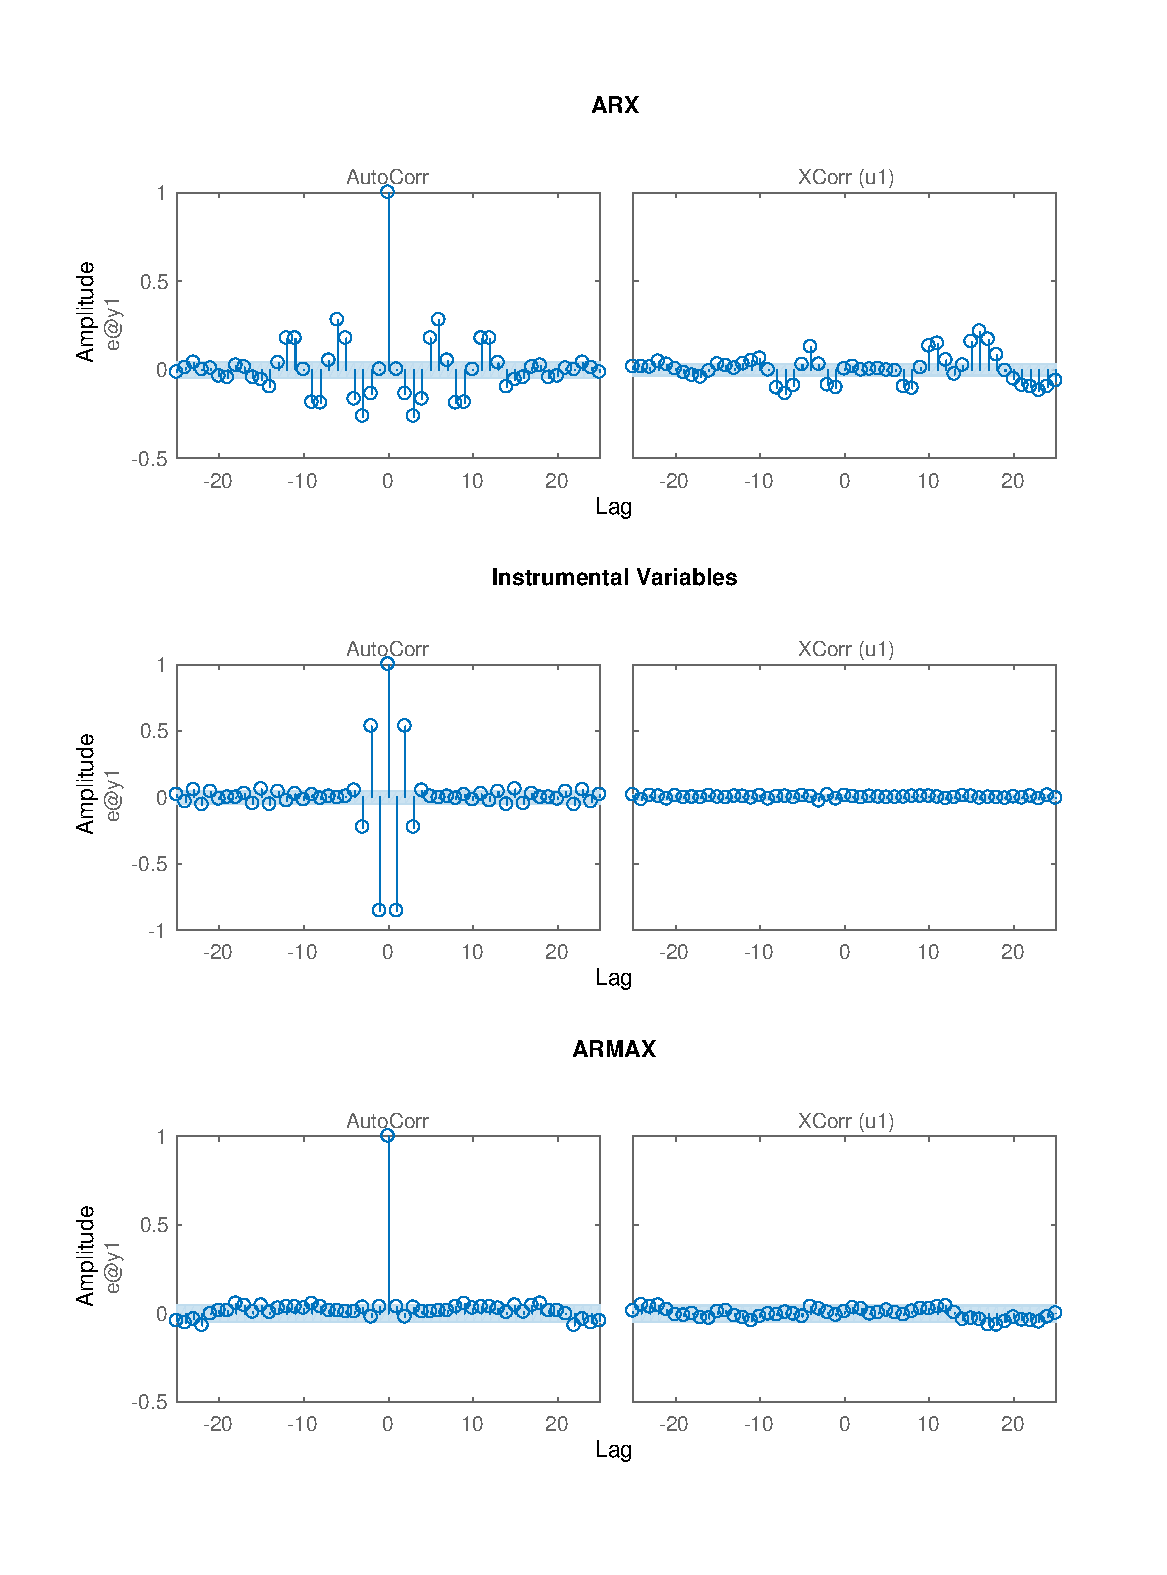
\includegraphics[width = 16cm]{images/4_resid_1}
%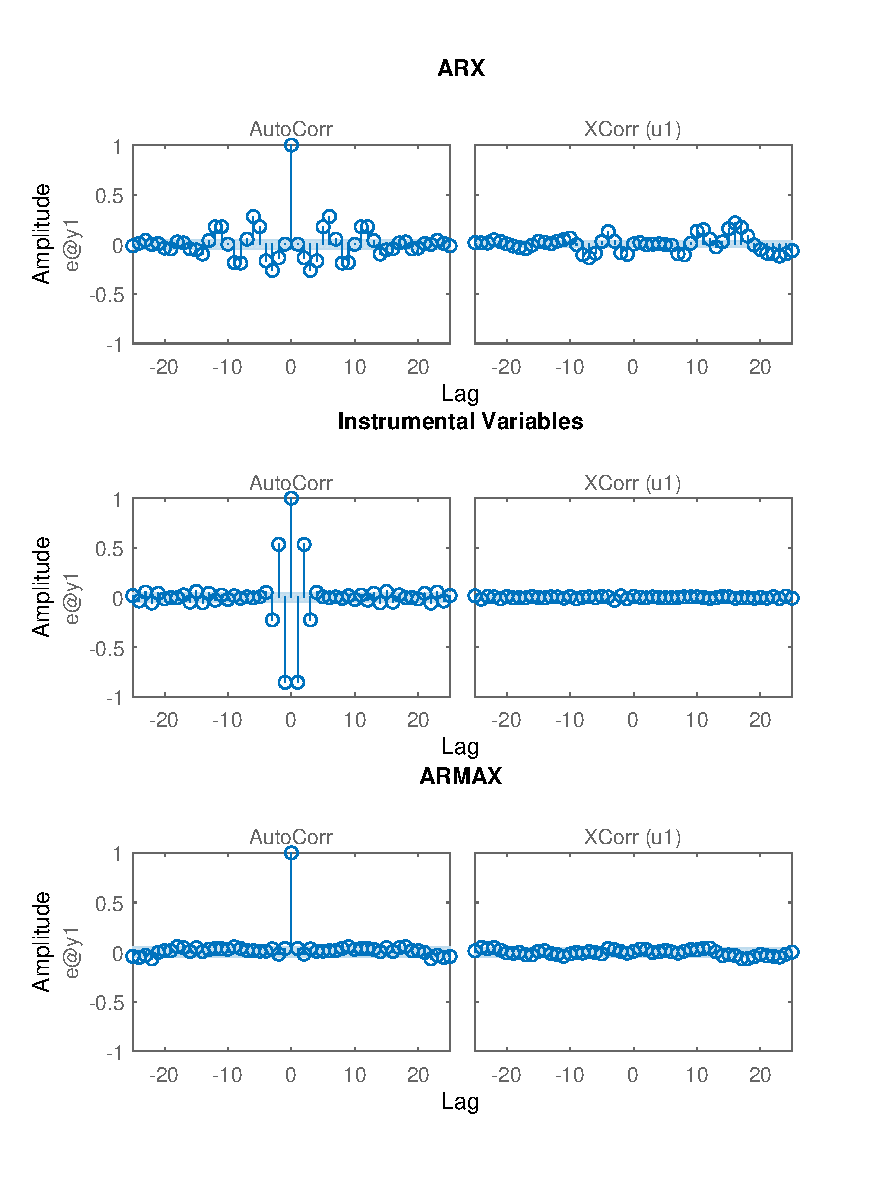
\includegraphics[width = 16cm]{images/system_resid1}
\caption{Whiteness test and uncorrelation test for the first three structures: the best result is given by the Instrumental Variables model}
\label{fig:sys_res1}
\end{figure}

\begin{figure}[H]
\centering
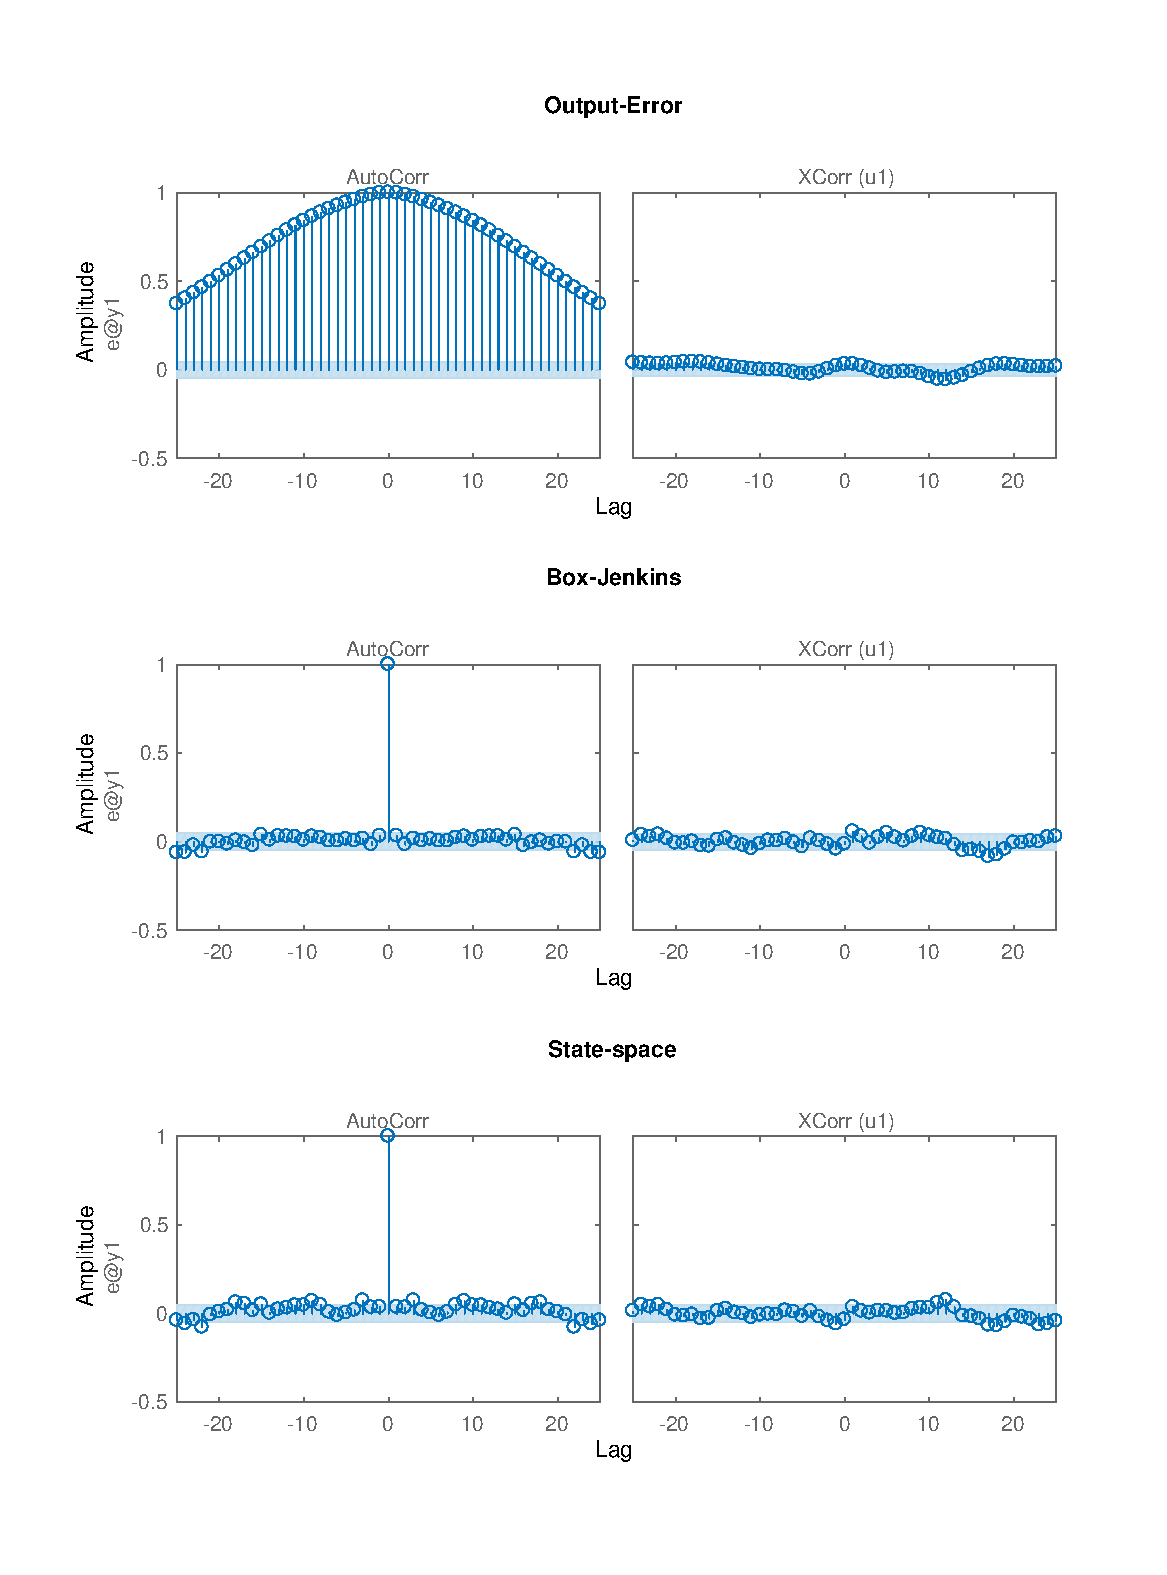
\includegraphics[width = 16cm]{images/4_resid_2}
%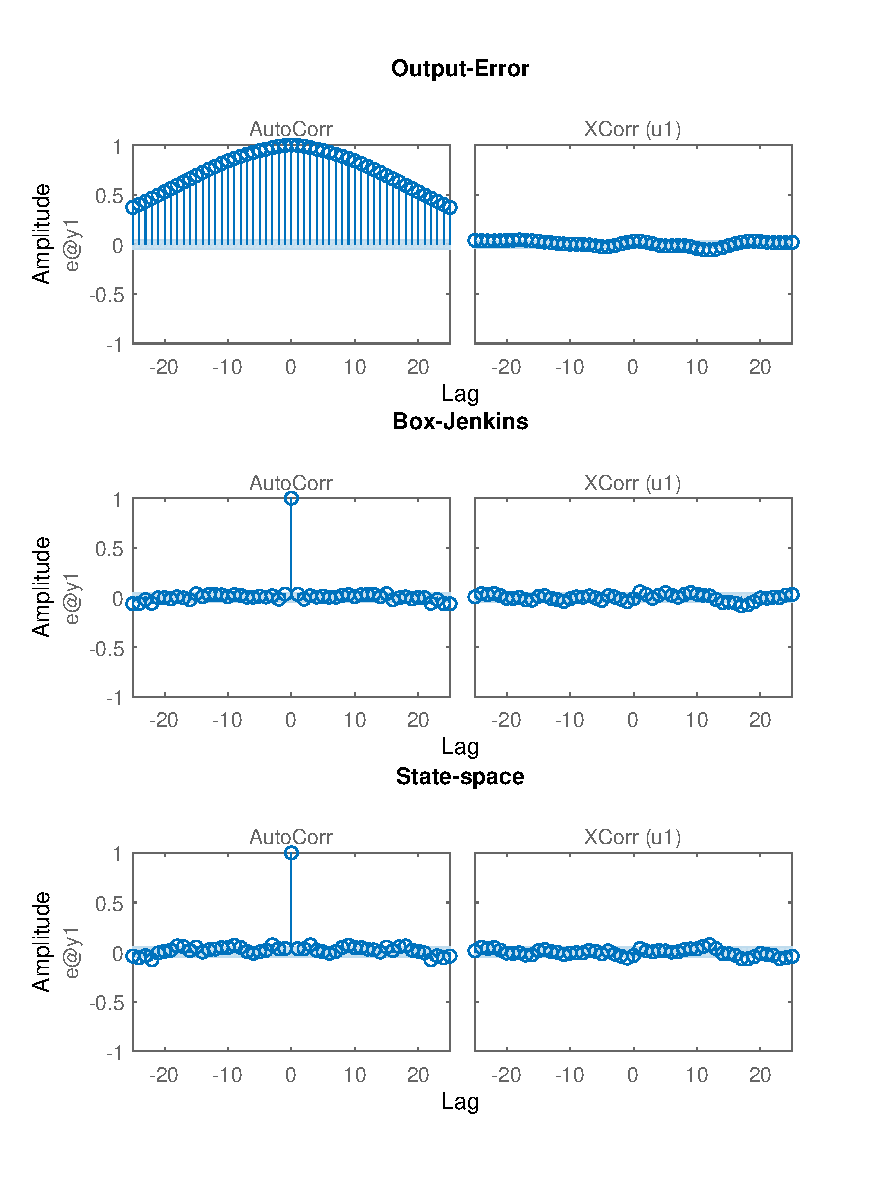
\includegraphics[width = 16cm]{images/system_resid2}
\caption{Whiteness test and uncorrelation test for the last three structures: the best result is given by the Box-Jenkins model, although the State-space model performs comparably well.
We notice that for the Output-Error structure the whiteness test is irrelevant as this structure does not contain a noise model. Also its main assumption that u(t) and the noise are uncorrelated is not satisfied. Thus we exclude the OE model.}
\label{fig:sys_res2}
\end{figure}

\begin{figure}[H]
\centering
\includegraphics[width = 16cm]{images/4_freq_domain_valid}
\caption{Frequency-domain validation: The models ARX, Output-Error and Instrumental Variables do not fit the second resonance frequency lobe. This is reason enough to discard them because it might be inside the operating frequency of the system.}
\label{fig:freq_valid}
\end{figure}

\begin{figure}[H]
\centering
\includegraphics[width = 16cm]{images/4_freq_visual_comp}
\caption{Closer look at frequency domain comparison of the different models (blue) with the spectral analysis model (red). We observe that most models have a $720^\circ$ phase lead to the actual model.}
\label{fig:freq_vsual_comp}
\end{figure}

\begin{figure}[H]
\centering
\includegraphics[width = 16cm]{images/4_freq_nk3_armax_bj}
\caption{When adding a delay $n_k = 3$ the phase lead disappears from the ARMAX and Box-Jenkins models, giving a relatively good fit in magnitude and phase. We could presume $n_k = 3$ gives a better fit even though during the order selection process we could rule out $n_k > 0$.}
\label{fig:freq_nk3_armax_bj}
\end{figure}

\begin{appendices}
\section{final\_project.m}
\label{app:final_project}
\lstinputlisting{final_project.m}

\section{frequency\_analysis.m}
\label{app:frequency_analysis}
\lstinputlisting{frequency_analysis.m}

\section{physical\_model.m}
\label{app:physical_model}
\lstinputlisting{physical_model.m}

\section{estimation.m}
\label{app:estimation}
\lstinputlisting{estimation.m}

\section{validation.m}
\label{app:validation}
\lstinputlisting{validation.m}

\section{intcor.m}
\label{app:intcor}
\lstinputlisting{intcor.m}

\end{appendices}

\end{document}
